\documentclass{beamer}
%\usetheme{Madrid} % My favorite!
%\usetheme{Boadilla} % Pretty neat, soft color.
%\usetheme{default}
%\usetheme{Warsaw}
%\usetheme{Bergen} % This template has nagivation on the left
\usetheme{Frankfurt} % Similar to the default 
%with an extra region at the top.
%\usecolortheme{seahorse} % Simple and clean template
%\usetheme{Darmstadt} % not so good
% Uncomment the following line if you want %
% page numbers and using Warsaw theme%
% \setbeamertemplate{footline}[page number]
%\setbeamercovered{transparent}


\newcommand{\argmin}{\operatornamewithlimits{arg\ min}}
\newcommand{\argmax}{\operatornamewithlimits{arg\ max}}
\newcommand\ville[1]{{\color{red} #1 }}
%    \mymarginpar{\raggedright\hbadness=10000\tiny\it #1\par}}

\newcommand{\myN}{\hbox{N\hspace*{-.9em}I\hspace*{.4em}}}
\newcommand{\myZ}{\hbox{Z}^+}
\newcommand{\R}{\mathbb{R}}
\renewcommand{\P}{\mathbb{P}}
\newcommand{\E}{\mathbb{E}}
\newcommand{\logit}{\text{logit}}


\setbeamercovered{invisible}
% To remove the navigation symbols from 
% the bottom of slides%
\setbeamertemplate{navigation symbols}{} 
%
\usepackage{graphicx}
\usepackage{amsmath,amsthm,amssymb}
\usepackage{subfigure}
%\usepackage{bm}         % For typesetting bold math (not \mathbold)
%\logo{\includegraphics[height=0.6cm]{yourlogo.eps}}
%
\title[Probability Aggregation]{Probability Aggregation: Dynamic Hierarchical Modeling of Sparse Expert Beliefs}
\author{Ville A. Satop\"a\"a,  Shane T. Jensen, Lyle H. Ungar, Barbara A. Mellers, Phil E. Tetlock}
\institute[University of  Pennsylvania]
{
University of Pennsylvania \\
\medskip
{\emph{satopaa@wharton.upenn.edu}}
}
\date{\today}
% \today will show current date. 
% Alternatively, you can specify a date.
%
\begin{document}
%
\begin{frame}
\titlepage
\end{frame}
%


\begin{frame}
\frametitle{Motivation}
\begin{enumerate}
\item Probability aggregation is important in decision-making (medical diagnosis, political and socio-economic foresight, meteorology, etc.)
\item Focus has been on developing one-time aggregation procedures that consult the expert's advice only once.
\item It is common for experts studying real problems to update their probability estimates over time.\\
\vspace{1em}
 $\Rightarrow$ Time-series probability aggregation
\end{enumerate}
\end{frame}



\begin{frame}
\frametitle{Data Example}

\begin{figure}[h!]
\centering
\vspace{-1.5em}
	
\includegraphics[width=  \textwidth]{LegendExamplePlot} % requires the graphicx package
\vspace{-1.5em}

\subfigure{
\hspace*{-1em}  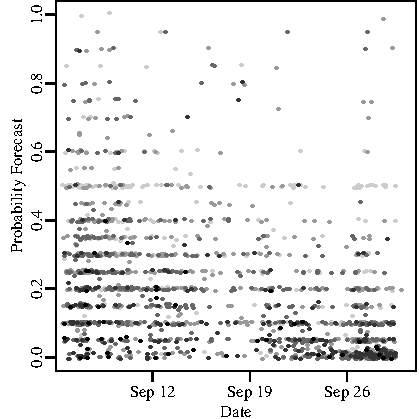
\includegraphics[width= 2.4in]{Figures/ExamplePlot2}
%\caption{\textit{Sample-Then-Optimize} with logarithmic score}
\label{Example2}
}

\caption{Will the Nikkei 225 index finish trading at or above 9,500 on 30 September 2011?}
\label{ExamplePlots}
\end{figure}
\end{frame}


\begin{frame}
\frametitle{Data Summary}
\begin{itemize}
\item $166$ questions about international political events.
\item Length of a question ranged from 4 to 418 days with an average of 73 days.
\item  $\sim 2,400$ experts participating.
\item On average, an expert participated in 55 questions.
\item On average, an expert gave 1 probability forecast per question.\\
\vspace{1em}
 $\Rightarrow$ The data is noisy and sparse.
\end{itemize}


\end{frame}


\begin{frame}
\frametitle{Data Example Returned}

\begin{figure}[h!]
\centering
\vspace{-1.5em}
	
\includegraphics[width=  \textwidth]{LegendExamplePlot} % requires the graphicx package
\vspace{-1.5em}

\subfigure{
\hspace*{-1em}  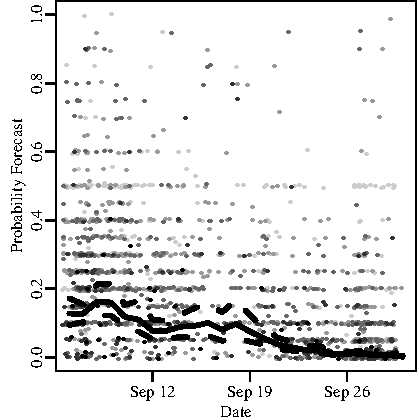
\includegraphics[width= 2.4in]{Figures/ExamplePlot2b}
%\caption{\textit{Sample-Then-Optimize} with logarithmic score}
\label{Example2}
}

\caption{Will the expansion of the European bailout fund be ratified by all 17 Eurozone nations before 1 November 2011?}
\label{ExamplePlots}
\end{figure}
\end{frame}



\begin{frame}
\frametitle{Research Goals}
\textbf{Core Research Problem:} Construct an \textit{interpretable} model for capturing a sharp and well-calibrated \textit{crowd belief} across time.
\vspace{1em}

\begin{block}{Calibration}
A probability forecast $p$ for the $k$th question is calibrated if $\P(Z_k = 1 | p) = \E[Z_k | p] = p$ almost surely.
\end{block}
\begin{block}{Sharpness}
A probability forecast $p$ is sharper than a probability forecast $q$ if $\E[(p-p_0)^2] > \E[(q-p_0)^2]$, where $p_0$ is the baseline probability for the $k$th question.
\end{block}

\end{frame}

\begin{frame}
\frametitle{Research Goals}
\textbf{Specific Research Objectives:}
\begin{enumerate}
\item Study bias across different levels of self-reported expertise.
\item Make predictions.
\item Give many question-specific quantities that have easy interpretations. 
\end{enumerate}
\vspace{1em}
\end{frame}
%

\begin{frame}
\frametitle{Model}
Our model is
\begin{eqnarray*}
\boldsymbol{Y}_{t,k}  &=& \text{log-odds for the $k$th question at time }t\\
\boldsymbol{Y}_{t,k}  &\sim&  \mathcal{N}_{n_k}\left( \boldsymbol{M}_k \boldsymbol{b} X_{t,k}, \sigma^2_k\boldsymbol{I}_{n_k} \right)\\
X_{t,k} &\sim& \mathcal{N} \left( \gamma_k X_{t-1,k}, \tau^2_k\right)
\end{eqnarray*}
where
\begin{itemize}
\item Only $\boldsymbol{Y}_{t,k}$ is observed.
\item $X_{t,k}$ is a sharp and well-calibrated logit-probability for the $k$th question at time $t$.
\item $\boldsymbol{b}$ is a vector of bias terms for the expertise groups.
\item $\gamma_k$ drives the hidden process toward extremes as $t \to T$. 
\item $\sigma^2_k$ quantifies random noise around expert forecasts. 
\item $\tau^2_k$ quantifies random shocks to the hidden process.
\end{itemize}

\end{frame}
%
\begin{frame}
\frametitle{Identifiability}
\textbf{This model is not identifiable:} Let $a$ be some non-negative constant. Then  $(\boldsymbol{b}/a, aX_{t,k}) \neq (\boldsymbol{b}, X_{t,k})$ give the same likelihood for $\boldsymbol{Y}_{t,k}$. 

\vspace{1em}
$\Rightarrow$ Parameter estimates drift!
\end{frame}
 
 \begin{frame}
\frametitle{Sample-And-Calibrate ($\text{SAC}_{LOG}$)}

\begin{block}{Sampling Step}
\begin{enumerate}
\item Fix $b_3 = 1$.
\item Sample constrained estimates: $\hat{X}_{t,k}(1)$, $\hat{\boldsymbol{b}}(1)$, etc.
\end{enumerate}
\end{block}

\begin{block}{Calibration Step}
\begin{enumerate}
\item Estimate $ \hat{b}_3 =  \argmax_{b \in \R / \{0\}} \sum_{k=1}^K \sum_{t=1}^{T_k}  S\left(Z_k, \hat{X}_{k,t}(1) / b \right)$
where $S$ is a strictly proper scoring rule such as the logarithmic score $Z \log\left(\logit^{-1}(X)\right) + (1-Z) \log\left(1-\logit^{-1}(X)\right)$

\item Adjust the constrained estimates:
\small
\vspace{-1em}
\begin{eqnarray}
 \hat{X}_{t,k}&=& \hat{X}_{k,t}(1) / \hat{b}_3 \nonumber\\
 \hat{\boldsymbol{b}}&=& \hat{\boldsymbol{b}}(1) \hat{b}_3 \nonumber\\
   \hat{\tau}_{k}^2&=& \hat{\tau}_{k}^2(1)/ \hat{b}_3^2\nonumber\\
  \hat{\sigma}_{k}^2&=& \hat{\sigma}_{k}^2(1)\nonumber\\
  \hat{\gamma}_{k}&=& \hat{\gamma}_{k}(1)\nonumber
\end{eqnarray}

\end{enumerate}
\end{block}
\end{frame}
 
 
\begin{frame}
\frametitle{Why Does This Work?}
\begin{itemize}
\item The maximization is really over different choices of $\hat{X}_{t,k}$. Since this process is assumed to be sharp and well-calibrated, it is natural to estimate it by maximizing a proper scoring rule.
\item If $S$ is the logarithmic scoring rule and the data is \textit{balanced}, then this process is approximately equivalent to Platt Calibration, which has been shown to yield good calibration under various modeling scenarios. \cite{platt1999probabilistic, niculescu2005obtaining}
\end{itemize}
\end{frame}
  
 
  
%  
%  \begin{frame}
%\frametitle{Balancing the Data}
%\begin{enumerate}
%\item Find a partition, $S_0$ and $S_1$, of the problem indices, $\{1, 2, \dots, 166\}$, such that the condition
%\begin{eqnarray*}
%\sum_{k \in S_0} T_k  = \sum_{k \in S_1} T_k  = \frac{1}{2}\sum_{k=1}^{166} T_k
%\end{eqnarray*}
%is as closely approximated as possible. 
%\item Let $\tilde{Z}_k = x$ with $x = 0,1$, and
%\begin{align*}
%\{\tilde{\boldsymbol{p}}_{t,k}\}_{t=1}^{T_k} &=  \begin{cases} 
%\{1-\boldsymbol{p}_{t,k}\}_{t=1}^{T_k} & \text{if } Z_k = 1-x\\
%\{\boldsymbol{p}_{t,k}\}_{t=1}^{T_k} & \text{if } Z_k = x 
%\end{cases}
%\end{align*}
%for $k \in S_x$. 
%\item $\left\{\left(\tilde{Z}_k, \{\tilde{\boldsymbol{p}}_{t,k} \}_{t=1}^{T_k}\right) \right\}_{k=1}^{166}$ is a balanced version of the data.
%\end{enumerate}
%\end{frame}
  
  
\begin{frame}
\frametitle{Calibration and Sharpness: in-sample}

\begin{figure}[h!]
\subfigure[\scriptsize SDLM In-Sample]{
\hspace*{-3em} 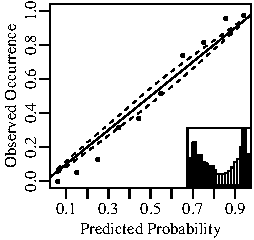
\includegraphics{Figures/CalibrationNONE10}
\label{CalibrationNONEa}
}
\subfigure[\scriptsize $\text{SAC}_{\text{LOG}}$ In-Sample]{
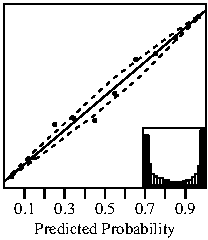
\includegraphics{Figures/CalibrationLOG10}
\label{CalibrationPLATTLOG10}
}
\caption[Optional caption for list of figures]{Comparing the approaches in terms of sharpness and calibration.}
\label{Calibration-Out}
\end{figure}

\end{frame}


\begin{frame}
\frametitle{Calibration and Sharpness: out-of-sample}

\begin{figure}[h!]
\subfigure[ \scriptsize SDLM Out-of-Sample]{
\hspace*{-3em} 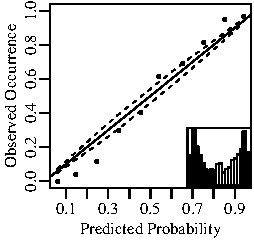
\includegraphics{Figures/CalibrationNONE}
\label{CalibrationNONEb}
}
\subfigure[ \scriptsize $\text{SAC}_{\text{LOG}}$ Out-of-Sample]{
 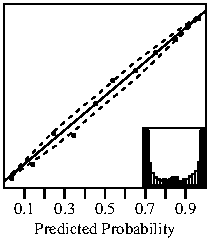
\includegraphics{Figures/CalibrationSTO-Log}
\label{CalibrationSTC-Log}
}
\caption[Optional caption for list of figures]{Comparing the approaches in terms of sharpness and calibration.}
\label{Calibration-Out}
\end{figure}
\end{frame}



\begin{frame}
\frametitle{Out-of-sample Prediction}
\begin{table}[htbp]
   \centering
   \scriptsize
      \begin{tabular}{l llll} % Column formatting, @{} suppresses leading/trailing space
 \multicolumn{5}{ c }{Scores by Day}\\
Model & \multicolumn{1}{ c }{All} & \multicolumn{1}{ c }{Short} & \multicolumn{1}{ c }{Medium} & \multicolumn{1}{ c }{Long}\\ \hline
SDLM & 0.100 (0.156) & 0.066 (0.116) & 0.098 (0.154) & 0.102 (0.157)\\ 
$\text{BSAC}_{\text{LOG}}$ & 0.097 (0.213) & \textbf{0.053} (0.147) & 0.100 (0.215) & 0.098 (0.215)\\ 
$\text{SAC}_{\text{BRI}}$ & 0.096 (0.190) & 0.056 (0.134) & 0.097 (0.190) & 0.098 (0.192)\\ 
$\text{SAC}_{\text{LOG}}$ & \textbf{0.096} (0.191) & 0.056 (0.134) & \textbf{0.096} (0.189) & \textbf{0.098} (0.193)\\ 
EWMBA & 0.102 (0.203) & 0.060 (0.124) & 0.110 (0.201) & 0.103 (0.206)\\ 
EWMLA & 0.102 (0.199) & 0.061 (0.130) & 0.111 (0.214) & 0.103 (0.200)\\ 
EWMA & 0.111 (0.142) & 0.089 (0.100) & 0.111 (0.136) & 0.112 (0.144)\\ 
&&&&\\
\multicolumn{5}{ c }{Scores by Problem}\\
Model & \multicolumn{1}{ c }{All} & \multicolumn{1}{ c }{Short} & \multicolumn{1}{ c }{Medium} & \multicolumn{1}{ c }{Long}\\ \hline
SDLM & 0.089 (0.116) & 0.064 (0.085) & 0.106 (0.141) & 0.092 (0.117)\\ 
$\text{BSAC}_{\text{LOG}}$ & 0.083 (0.160) & \textbf{0.052} (0.103) & 0.110 (0.198) & 0.085 (0.162)\\ 
$\text{SAC}_{\text{BRI}}$& 0.083 (0.142) & 0.055 (0.096) & 0.106 (0.174) & 0.085 (0.144)\\ 
$\text{SAC}_{\text{LOG}}$ & \textbf{0.082} (0.142) & 0.055 (0.096) & \textbf{0.105} (0.174) & \textbf{0.085} (0.144)\\ 
EWMBA & 0.090 (0.156) & 0.063 (0.101) & 0.118 (0.186) & 0.091 (0.161)\\ 
EWMLA & 0.090 (0.159) & 0.064 (0.109) & 0.120 (0.200) & 0.090 (0.159)\\ 
EWMA & 0.104 (0.105) & 0.092 (0.081) & 0.119 (0.125) & 0.103 (0.107)\\ 
   \end{tabular}
   \caption{Brier Scores based on 10-fold cross-validation.}
   \label{prediction}
\end{table}

\end{frame}

\begin{frame}
\frametitle{Group-level bias}
\vspace{-0.9em}
\begin{figure}[!ht]
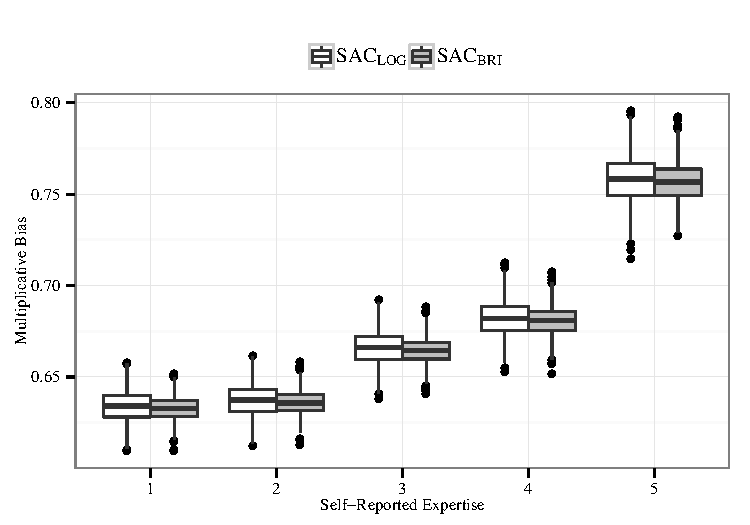
\includegraphics[width = 4in]{Figures/BiasesBoxplots}
\label{BiasesLOGBoxplots}
\vspace{-1em}
\caption[Optional caption for list of figures]{Comparing the bias-levels across self-reported expertise under different approaches.}
\label{Biases}
\end{figure}
\end{frame}

\begin{frame}
\frametitle{Conclusion}
\begin{itemize}
\item Extended probability aggregation towards unexplored areas.
\item Gave an interpretable model that offers a solution to the main problems in time-series probability aggregation.
\item Applied this to a large probability forecasting dataset.
\item Many future extensions.
\end{itemize}

\end{frame}



\begin{frame}
\centering 
\hspace{12em}Questions?
\end{frame}

 
       \begin{frame}
\frametitle{References}
\tiny
 \bibliographystyle{plainnat}
%\bibliographystyle{imsart-nameyear}
\bibliography{biblio}		% expects file "myrefs.bib"
\end{frame}



\end{document} 
